In cui si descrive la progettazione del software a un più basso livello: scelte progettuali, tecnologie e linguaggi adottati.

\section{Greenbone OpenVAS}
Come backend di scansione per il sistema, inizialmente si è optato per interfacciarsi a \textbf{Greenbone OpenVAS}.

\section{Base di dati}
Il framework di Greenbone già include un suo database interno per la gestione degli utenti e dei ruoli associati ad essi, così come per le scansioni, i risultati e la reportistica. Inoltre, gran parte della logica di business rilevante è già definita e può essere personalizzata con un sistema di permessi abbastanza preciso e granulare, rendendo possibile adattarla facilmente ai nostri scopi.

Per questo motivo, si è deciso di non introdurre ridondanza e complessità con un ulteriore database, preferendo invece rimanere aderenti alla base di dati esistente, effettivamente sposando in tutto e per tutto la struttura dei dati proposta da Greenbone.

\subsection{Schema dei dati originale}
Lo schema dei dati proposto da Greenbone è strutturato come illustrato in figura \ref{er-crow}\footnote{Si noti che il diagramma ER qui realizzato rappresenta solamente le entità d'interesse considerate per il progetto: il reale database contiene uno schema più esteso e maggiormente interconnesso.}. In particolare:
\begin{itemize}
    \item Una \textbf{Task} rappresenta una scansione predisposta e configurata da un utente (\textbf{User}).
    \item Un utente appartiene ad uno o più ruoli (\textbf{Role}) (nel nostro caso specifico apparterrà sempre a uno ed un solo ruolo). Ogni ruolo inoltre può possedere dei permessi (\textbf{Permission}).
    \item Allo stesso modo, un utente appartiene ad uno o più gruppi (\textbf{Group}) (nel nostro caso specifico l'utente apparterrà al massimo sempre ad un gruppo). Anche i gruppi sono associati a dei permessi.
    \item I permessi sono espressi da un \emph{soggetto} su una \emph{risorsa}. Sia \emph{risorsa} che \emph{soggetto} rappresentano una qualunque entità del sistema, di qualunque tipo.
    \item Ad ogni risorsa possono essere associati uno o più \textbf{Tag} in forma di coppie nome valore. Nel nostro caso useremo questi tag per esprimere la quota dell'utente e pertanto saranno usati solo come decorazione ulteriore dell'entità utente.
    \item Un task è associato a delle preferenze di scansione (\textbf{Preference}). Queste preferenze sono espresse in XML e rappresentano dei dettagli di funzionamento, tra cui soprattutto la \emph{retention policy} dei rapporti generati.
    \item Ogni task è associato a una configurazione di scansione (\textbf{Config}). Questa prescrive in buona sostanza quali VT / NVT vengono eseguiti dalla scansione. Si noti che Greenbone esternamente distingue tra due tipi di configurazione di scansione:
    \begin{itemize}
        \item \emph{Scan config}: ovvero una semplice configurazione definita da un utente umano.
        \item \emph{Policy}: ovvero una scansione prescritta a norma di legge o in ottemperanza a qualche specifico standard. Queste ovviamente andrebbero lasciate così come fornite dal feed.
    \end{itemize}
    Questa distinzione internamente non è gestita con una separazione in entità distinte, come si può vedere dallo schema (allo stesso modo il progetto realizzato non fa distinzioni tra le due tipologie di configurazioni, internamente).
    \item Ogni scansione viene eseguita su un bersaglio specifico (\textbf{Target}). Un bersaglio di Greenbone OpenVAS specifica uno o più nodi di rete da scansionare, dettagliando anche eventuali credenziali di rete da usare per simulare un attacco di tipo \emph{white box}\footnote{In un attacco / test di tipo \emph{white box} l'attaccante è a disposizione di conoscenza rilevante e approfondita circa l'infrastruttura bersaglio. In un test \emph{black box} invece non viene fornito nessun aiuto / informazione, mentre in un \emph{gray box} vi è una via di mezzo, rappresentando di fatto la tipologia d'attacco più comune.} e le porte da considerare nella scansione.
    \begin{itemize}
        \item Le porte sono definite tramite un'entità \textbf{Portlist} associata. Questa internamente definisce le singole porte in modo efficiente tramite dei \emph{range} divisi per tipo (UDP o TCP).
    \end{itemize}
    \item Un task è eseguito da uno \textbf{Scanner}. In pratica questo è quasi sempre OpenVAS, ma Greenbone mette a disposizione anche uno scanner fittizio detto \textbf{CVE}, già dettagliato in \ref{cve}.
    \item Un task può essere associato anche ad una \textbf{Schedule}, che ne definisce un'eventuale esecuzione futura / ritardata e/o periodica / ricorrente. A basso livello la schedule è espressa tramite standard \textbf{iCalendar}.
    \item Un task contiene informazioni relative alla sua esecuzione, come il suo stato (in pausa, in esecuzione, in coda, fallita per errore, ecc.) e la percentuale di completamento.
    \item Infine, un task genera uno o più \textbf{Report}. Questi recano informazioni sul periodo temporale a cui sono riferiti e sul numero delle vulnerabilità trovate, nonché la loro severità. Le vulnerabilità si dividono in:
    \begin{itemize}
        \item \textbf{Falsi positivi}: vulnerabilità rilevate dal processo di scansione, ma che lo scanner è riuscito ad identificare autonomamente come falsi positivi.
        \item \textbf{Log}: spesso non sono vere e proprie vulnerabilità, ma semplici informazioni sul sistema di utilità quasi nulla. Alcune di queste sono solitamente disabilitate dagli amministratori di OpenVAS poiché inutilmente paranoiche.
        \item \textbf{Info}: vulnerabilità di basso livello, spesso che forniscono solo informazioni sul sistema, di utilità non nulla.
        \item \textbf{Warning}: vulnerabilità di medio livello, come vecchi standard crittografici ancora in uso, Denial of Service, ecc.
        \item \textbf{Hole / High / Critical}: vulnerabilità o problematiche ad alto livello di rischio e danno potenziale, come RCE, Privilege Escalation, EOL, ecc.
    \end{itemize}
    \item Un rapporto organizza quanto trovato in ``risultati'' (\textbf{Result}). Queste entità contengono metadati che descrivono testualmente la vulnerabilità, l'eventuale soluzione e forniscono gli riferimenti a CVE, CVSS e CPE relativi.
    \item Inoltre, l'esecuzione di un task rivela tutta una serie di \textbf{Asset} che vengono scoperti e inventariati durante la realizzazione del rapporto. Questi sono principalmente:
    \begin{itemize}
        \item \textbf{Host}, ovvero macchine fisiche o virtuali (questo comportamento può essere personalizzato come opzione dello scanner).
        \item Sistemi operativi (\textbf{OS}), con vari gradi di precisione nel loro processo di \emph{fingerprinting}.
    \end{itemize}
\end{itemize}

\begin{figure}
    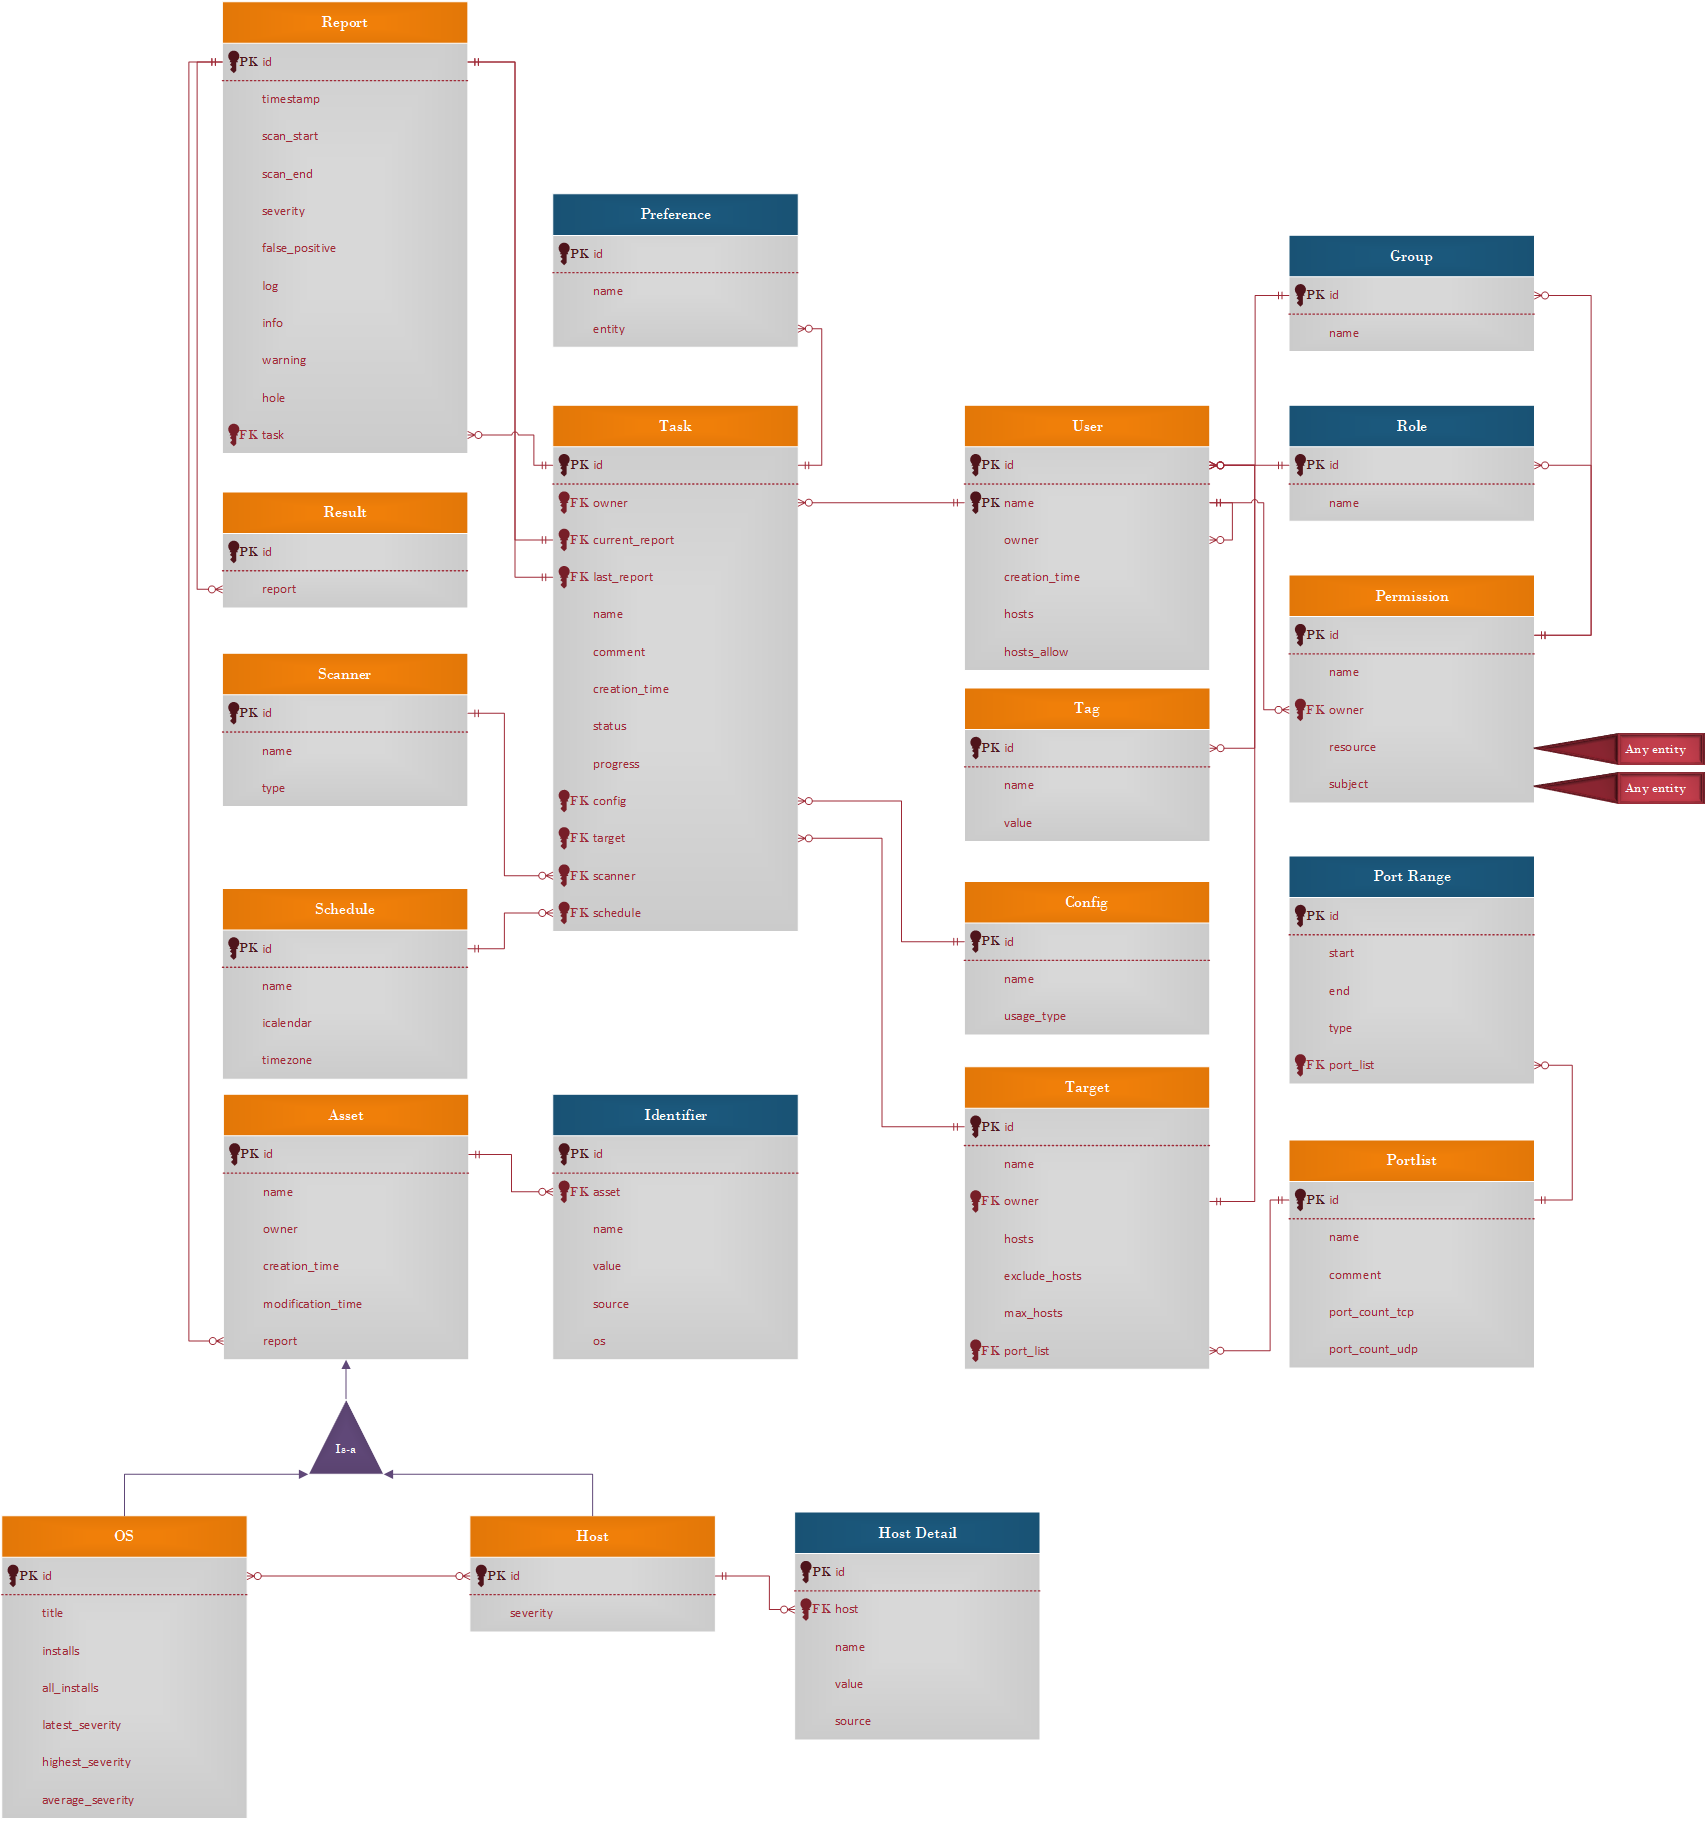
\includegraphics[width=\textwidth]{img/er_crow.png}
    \caption{Schema dei dati d'interesse di GVM}
    \label{er-crow}
\end{figure}

\section{Architettura}
Come anticipato in \ref{microservices}, in fase di analisi è emersa la necessità di realizzare sin dall'inizio un sistema modulare e disaccoppiato. Da un punto di vista puramente teorico e di architettura si deducono i seguenti sistemi con le seguenti funzionalità:
\begin{itemize}
    \item Uno o più backend di scansione. Come già detto, si vuole usare \textbf{OpenVAS} per questo componente, riservando l'integrazione con altri backend a sviluppi futuri.
    \item Un sistema che fa da interconnessione e adattatore tra il backend di scansione, introducendo un livello di indirezione e fornendo funzionalità ad un sistema \emph{user-facing} attraverso un'API unificata.
    \item Il sistema di interfaccia, che si interconnette con l'adattatore di cui sopra per fornire un \emph{frontend} facilitato e moderno per l'uso da parte dell'utente finale.
\end{itemize}
Tenuto conto delle moderne tendenze di sviluppo, dei framework supportati e della necessità di avere un sistema \emph{cross-platform}, si è deciso per sviluppare gli ultimi due sistemi tramite un'\textbf{applicazione web} composta da due parti distinte ricalcanti rispettivamente gli scopi dei sistemi sopracitati:
\begin{itemize}
    \item Un \emph{backend} realizzato in forma di \textbf{REST API}. Questo si appoggerà sul database interno di Greenbone OpenVAS indirettamente attraverso il protocollo GMP.
    \item Un \emph{frontend} realizzato in forma di \textbf{SPA}, che sfrutta il backend per interagire con il sistema di scansione.
\end{itemize}

\section{REST API di Backend}
REST è un paradigma ormai molto popolare di sviluppo delle API web. Una REST API spesso non implementa tutto lo standard REST, ma quanto segue sono le specifiche più comuni e popolarmente identificate come minime:
\begin{itemize}
    \item \textbf{Stateless}: ogni richiesta del client deve contenere tutte e sole le informazioni necessarie a comprendere la richiesta. In teoria il server non dovrebbe neanche mantenere stato e gestire l'autenticazione mediante token di accesso, ma in pratica questo aspetto dello standard è modificato per usare i cookie di sessione, specie quando la REST API è consumata esclusivamente da client web come una Single Page Application (scenario sempre più comune).
    \item Le entità del sistema sono rappresentate come \textbf{risorse}, identificate dallo URL e da formati specifici come JSON (usato per questo progetto) o XML.
    \item La semantica delle operazioni eseguibili sulle risorse è sottintesa dai \textbf{metodi HTTP} utilizzati (GET per ottenere la/e risorsa/e, POST per crearne di nuova, PUT / PATCH per aggiornare le risorse, DELETE per rimuoverne).
\end{itemize}

\subsection{Linguaggio di programmazione}
Dall'analisi delle librerie offerte da Greenbone per l'interconnessione dei suoi sistemi, effettuata in \ref{libraries}, emerge chiaramente la superiorità in quest'ambito del linguaggio \textbf{Python}, semplicemente per la presenza di una libreria software ufficialmente manutenuta e supportata.

Infatti, utilizzare un linguaggio di programmazione diverso dal Python imporrebbe la necessità di sviluppare e manutenere in proprio una libreria che faccia da \emph{client} per la socket UNIX, dialogando con il protocollo GMP, realizzando di fatto un doppione di una libreria già esistente, solo per un altro linguaggio.

Inoltre, sarebbe necessario implementare da zero lo schema dei dati descritto dal protocollo, aggiungere funzionalità di \emph{parsing}, controllo degli errori, ma soprattutto andrebbe aggiornando di volta in volta di pari passo con gli aggiornamenti al protocollo GMP.

Per tutti questi motivi, si è considerato l'uso di \texttt{python-gvm} come una scelta quasi obbligata. L'unico vantaggio che poteva portare l'uso di una libreria sviluppata indipendentemente era l'integrazione diretta di una traduzione dal linguaggio XML in una struttura dati più ricca, di fatto realizzando un \textbf{ORM} a livello di libreria di interconnessione con la base dati (qua indirettamente rappresentata dal protocollo GMP). Questa funzione di traduzione non è implementata dalla libreria \texttt{python-gvm}, rendendo di fatto obbligatoria una piccola parte di gestione aggiuntiva a livello di modello\footnote{``Modello'' inteso nel senso del \emph{design pattern} \textbf{MVC, Model View Controller}, secondo il quale un'applicazione può essere scomposta in una parte di accesso e gestione dei dati (\emph{model}) e una parte di interfaccia (\emph{view}), mediate unicamente da un livello di interconnessione il più possibile semplice e minimale (\emph{controller}).} dei dati.

\subsection{Framework}
Per un progetto destinato ad un uso professionale è imperativo utilizzare un \emph{framework}, per garantire soprattutto sicurezza, facilità di manutenibilità e anche di sviluppo.

Avendo scelto il linguaggio Python, emergono soprattutto tre framework sufficientemente manutenuti e utilizzati da poter essere comparati:
\begin{itemize}
    \item \textbf{Django} è un framework web ad alto livello che incoraggia lo sviluppo rapido e un design pulito e pragmatico. Di fatto è il framework web full-stack più popolare in ambito Python, comparabile con Laravel e Ruby on Rails per gli ecosistemi rispettivamente PHP e Ruby.
    
    Django offre una serie di funzionalità integrate per accelerare lo sviluppo, come un proprio ORM (Object-Relational Mapping), un sistema di autenticazione, un pannello di amministrazione automatico e strumenti per la gestione delle migrazioni del database. Utilizza un'architettura Model-Template-View, che separa la logica di business dalla presentazione in modo simile all'architettura MVC, e include protezioni contro attacchi comuni come SQL injection, cross-site scripting (XSS) e cross-site request forgery (CSRF).
    \item \textbf{Flask} è un micro-framework leggero e flessibile per Python, progettato per essere semplice e facile da estendere. Esso fornisce solo le funzionalità di base, lasciando agli sviluppatori la libertà di scegliere individualmente le singole librerie e gli strumenti da utilizzare. La sua architettura minimalista lo rende ideale per progetti più piccoli o per applicazioni che richiedono una personalizzazione significativa. Grazie alla sua semplicità, è spesso utilizzato per sviluppare prototipi, applicazioni minimali o dal design particolarmente esotico, e può essere facilmente esteso con numerosi plugin e librerie di terze parti.
    \item \textbf{FastAPI} è un framework moderno e veloce per costruire API con Python 3.6+ fortemente basato sullo standard \textbf{OpenAPI}. È progettato per essere altamente performante e facile da usare. FastAPI poggia sul framework web Starlette e la libreria Pydantic, che tramite le annotazioni di Python fornisce di default una validazione automatica dei dati. Inoltre, FastAPI supporta la generazione automatica e auto-aggiornante di una documentazione interattiva delle API sviluppata, grazie allo standard OpenAPI e Swagger UI o ReDoc. Infine, supporta anche la programmazione asincrona, a differenza di tutti gli altri framework.
\end{itemize}
In questo progetto si è deciso per l'adozione del framework Flask, sulla base di una serie di considerazioni tecniche e pratiche che ne evidenziano l'idoneità rispetto alle altre opzioni disponibili.

Infatti, sebbene Django offra un ecosistema robusto e completo, è principalmente orientato verso applicazioni full-stack monolitiche e non si presta in modo ottimale alla creazione di REST API, nonostante l'esistenza di Django Rest Framework. Quest'ultimo, infatti, suggerisce che il framework non è stato concepito in partenza con questo scopo primario in mente.

D'altra parte, FastAPI è un framework moderno progettato specificamente per la creazione di REST API, presentandosi sullo spettro opposto rispetto a Django, ma presenta altre limitazioni significative. La mancanza di un'API pubblica per i suoi componenti rende il progetto meno affidabile nel lungo termine, specialmente per applicazioni di grande rilevanza. Inoltre, la gestione della codebase lasciata in gran parte nelle mani di un singolo sviluppatore solleva interrogativi sulla sostenibilità del progetto.

Flask, al contrario, si distingue per la sua flessibilità rendendolo particolarmente adatto per il caso specifico, che non prevedendo un database risulta abbastanza peculiare. Tra l'altro, sotto questo aspetto si discosta nettamente da FastAPI e Django, che possono risultare eccessivamente rigidi e guidati.

Flask consente di plasmare l'applicazione secondo le specifiche esigenze del progetto, sfruttando un ecosistema di estensioni molto florido. Segue ora in che modo queste estensioni sono state scelte a livello architetturale.

\subsection{Validazione dei dati e API REST}
Questo consente tra l'altro di replicare le funzionalità più avanzate di FastAPI, come la validazione dei dati e la generazione automatica della documentazione.

Queste funzionalità sono replicate in Flask attraverso l'uso di plugin ben mantenuti dalla comunità:
\begin{itemize}
    \item La validazione dei dati è gestita con la libreria \textbf{Marshmallow}, integrata in Flask con un'estensione che funge da collante tra le librerie.
    \item \textbf{APIFlask} invece è un plugin / framework secondario che funge da wrapper rispetto a Flask. Il suo scopo è facilitare la creazione di API, ma integrano anche la generazione automatica di specifiche OpenAPI e documentazione interattiva tramite Swagger UI, ReDoc e non solo.
\end{itemize}

\subsection{Autenticazione e sicurezza}
La sicurezza del backend di una REST API è un aspetto fondamentale da considerare durante lo sviluppo di un'applicazione web e questa non fa eccezione. Esistono diversi metodi per autenticare una REST API, tra cui l'uso di \textbf{token di accesso} e \textbf{cookie di sessione}. Ogni approccio presenta vantaggi e svantaggi in termini di facilità d'uso e sicurezza, e la scelta del metodo più appropriato dipende dalle specifiche esigenze del progetto.

Nel contesto di questo progetto, è stata presa la decisione di utilizzare i cookie di sessione per l'autenticazione. Questo metodo si distingue per la sua semplicità e sicurezza:
\begin{itemize}
    \item A differenza dei token di accesso, che devono essere inclusi manualmente in ogni richiesta HTTP, \textbf{i cookie di sessione vengono gestiti automaticamente dal browser}. Ciò significa che il programmatore non deve preoccuparsi di inviare il token ad ogni richiesta, semplificando notevolmente lo sviluppo dell'applicazione.
    \item Inoltre, i cookie di sessione possono essere configurati con attributi di sicurezza come \texttt{Secure}, \texttt{HttpOnly} e \texttt{SameSite}:
    \begin{itemize}
        \item L'attributo \texttt{Secure} garantisce che il cookie venga trasmesso solo su connessioni HTTPS. Questo significa che le informazioni contenute nel cookie non possono essere intercettate durante il transito tra il client e il server, proteggendo così i dati sensibili da attacchi di tipo man-in-the-middle. Senza questo attributo, i cookie potrebbero essere inviati anche su connessioni non sicure, esponendo le informazioni a potenziali attaccanti.
        \item L'attributo \texttt{HttpOnly} impedisce l'accesso al cookie tramite JavaScript. Questo è particolarmente importante per proteggere i cookie da attacchi di cross-site scripting (XSS), in cui un attaccante potrebbe tentare di eseguire codice malevolo nel contesto del browser dell'utente. Se un cookie è contrassegnato come HttpOnly, anche se un attaccante riesce a iniettare codice JavaScript nella pagina, non sarà in grado di accedere al contenuto del cookie, riducendo significativamente il rischio di furto di sessione.
        
        Se invece si usano i token è necessario maneggiarli con JavaScript per introdurli nelle richieste, di fatto introducendo un'ulteriore superficie d'attacco (XSS, appunto). Una mitigazione sarebbe istruire il server per fornire il token in un cookie \texttt{HttpOnly}, ma non tutte le librerie di gestione dei token supportano trasparentemente questa pratica, rendendo necessaria l'implementazione di codice ``collante'' che introduce ulteriori rischi di security. Sotto questo punto di vista la natura personalizzabile e spoglia di Flask ha favorito la nascita di un'ecosistema frammentato e senza ancora una libreria di sicurezza standard.
        \item Infine, l'attributo \texttt{SameSite} offre una protezione contro attacchi di cross-site request forgery (CSRF). Questo attributo consente di specificare se il cookie deve essere inviato con richieste provenienti da siti esterni. Impostando SameSite su \texttt{Strict} o \texttt{Lax}, il cookie non verrà inviato con richieste che non provengono dallo stesso dominio, limitando così le possibilità di attacchi CSRF.
        
        Nel progetto in oggetto si è comunque implementato un token CSRF per ulteriore scrupolo, grazie al framework \texttt{WTForms} sviluppato dai manutentori di Flask.
    \end{itemize}
    \item La possibilità di effettuare il logout in modo semplice e diretto rappresenta un ulteriore vantaggio di questo approccio, senza la necessità di dover introdurre \emph{blacklist} o simili stratagemmi, pratica invece comune quando si lavora con token web.
\end{itemize}

Sebbene l'uso di token di accesso offra vantaggi significativi, come una maggiore scalabilità in contesti distribuiti e la necessità di supportare client diversi da un browser, queste problematiche sono considerate distanti nel progetto qui considerato e potrebbero per giunta non rivelarsi mai rilevanti. L'autenticazione web, invece, è un aspetto certo e inevitabile, e la scelta di cookie di sessione si allinea perfettamente con le esigenze attuali del progetto.

Tuttavia, è importante notare che nulla vieta di adottare un approccio ibrido, simile a quello per esempio della popolare libreria ufficiale Sanctum del framework Laravel, che supporta entrambi i sistemi di autenticazione, cookie e token. In questo modo, si utilizzano i cookie di sessione per le applicazioni web a pagina singola (SPA), come nel nostro caso, e i token di accesso rimarrebbero a disposizione degli altri client, come le applicazioni mobili. Questa strategia consentirebbe di sfruttare i vantaggi di entrambi i metodi, garantendo una maggiore flessibilità e adattabilità alle diverse esigenze degli utenti e dei dispositivi.

La libreria scelta per gestire questo ambito è la popolare e open-source \texttt{flask-login}.

\subsection{Gestione sessioni}
La gestione delle sessioni è un aspetto cruciale nello sviluppo di applicazioni web, e la scelta del metodo di memorizzazione delle sessioni può influenzare significativamente la sicurezza e le prestazioni dell'applicazione. Di default, Flask utilizza esclusivamente sessioni \emph{client-side}, il che significa che i dati della sessione vengono memorizzati direttamente nei cookie del browser dell'utente. Questo approccio comporta che ogni volta che il client effettua una richiesta al server, il cookie contenente le informazioni della sessione viene inviato insieme alla richiesta. Sebbene questo metodo possa sembrare semplice e immediato, presenta alcune limitazioni, tra cui il fatto che i dati sensibili sono visibili a chiunque, siccome la crittografia usata per il cookie non garantisce la confidenzialità dei dati al suo interno, ma solo la sua integrità.

Per superare queste limitazioni, si è deciso per l'uso di \texttt{flask-session}, una libreria che consente a Flask di gestire sessioni \emph{server-side}. Con le sessioni server-side, i dati della sessione vengono memorizzati sul server, mentre il client riceve nel cookie solamente un identificatore univoco della sessione. Questo approccio offre numerosi vantaggi in termini di sicurezza, poiché i dati sensibili non vengono mai esposti al client. Inoltre, consente una gestione più efficiente delle sessioni, poiché il server può mantenere lo stato dell'utente senza dover inviare continuamente informazioni sensibili attraverso la rete.
Rimane comunque necessario difendersi da attacchi come la \textbf{Session Fixation}; questa parte è approfondita in \ref{session-fixation}.

Per implementare le sessioni \emph{server-side} di Flask Session, si è deciso per l'uso di \textbf{Redis}, un sistema di archiviazione in memoria, strutturato come un database chiave-valore, noto per la sua velocità e leggerezza. È particolarmente adatto per la gestione delle sessioni o di piccole \emph{cache}, poiché consente un accesso rapido e scalabile ai dati memorizzati. Inoltre, Redis è ampiamente supportato dalla libreria scelta ed è attivamente sviluppato, il che scongiura rischi di integrazione.

\subsection{CORS e DotEnv}
Durante lo sviluppo locale dell'applicazione, è emersa la necessità di gestire le richieste in regime di \textbf{Cross-Origin Resource Sharing (CORS)}. CORS è un meccanismo di sicurezza implementato nei browser che consente o limita le richieste effettuate da un'origine (domain) a un'altra. Questo è particolarmente rilevante quando si sviluppano applicazioni web che interagiscono con API o risorse ospitate su domini diversi, e negli ambienti di sviluppo è comune. Senza una corretta configurazione di CORS, il browser bloccherebbe automaticamente le richieste provenienti da origini non autorizzate, impedendo così il corretto funzionamento dell'applicazione. Per affrontare questa problematica, è stata utilizzata un'estensione di Flask specificamente progettata per gestire CORS (\texttt{Flask-CORS}), che consente di configurare facilmente le politiche di accesso e di specificare quali origini sono autorizzate a interagire con l'API.

In aggiunta alla gestione di CORS, è fondamentale considerare che molte funzionalità dell'applicazione possono variare a seconda dell'ambiente in cui si trova (come CORS stesso; come si vedrà nell'installazione finale dettagliata in \ref{deployment} non sarà necessario usarlo). Ad esempio, alcune funzionalità potrebbero essere attivate in fase di sviluppo, ma disattivate in produzione per motivi di sicurezza o prestazioni. Per gestire in modo efficace queste configurazioni environment-dependent, è stato adottato lo standard \textbf{DotEnv}. DotEnv è una convenzione per la gestione delle variabili di ambiente, che consente di definire configurazioni specifiche per ciascun ambiente in file di testo semplici, solitamente denominati \texttt{.env}. Questi file contengono coppie chiave-valore che possono essere facilmente lette dall'applicazione al momento dell'avvio.

L'integrazione di DotEnv con Flask è facilitata da un'altra estensione, \texttt{Flask-DotEnv}, che consente di caricare automaticamente le variabili di ambiente definite nel file .env all'interno dell'applicazione. Questo approccio non solo semplifica la gestione delle configurazioni, ma migliora anche la sicurezza, poiché consente di mantenere informazioni sensibili, come chiavi API e credenziali di accesso, al di fuori del codice sorgente (i file .env non sono mai aggiunti al sistema di controllo della versione, ma solo una loro versione di esempio, nel caso specifico denominata \texttt{.env.example}). In questo modo, è possibile evitare di esporre dati sensibili in repository pubblici o in ambienti di sviluppo condivisi.

\section{SPA di Frontend}
Una \textbf{SPA (Single Page Application)} è un tipo di applicazione web che carica una singola pagina HTML e aggiorna dinamicamente il contenuto in risposta alle interazioni dell'utente, senza la necessità di ricaricare l'intera pagina. Questo approccio migliora notevolmente l'esperienza utente, poiché consente transizioni più fluide e tempi di risposta più rapidi, rendendo l'applicazione più reattiva e simile a un'applicazione desktop, cosa desiderata per il progetto in questione.

\subsection{Scelta tra SPA e rendering ibrido}
In alternativa alla scelta di sviluppare una SPA, si sarebbe potuto considerare un approccio di rendering ibrido, come quello offerto da Inertia.js o librerie simili. Questo tipo di soluzione consente di combinare le caratteristiche delle applicazioni tradizionali con quelle delle SPA, permettendo di costruire interfacce utente moderne senza dover gestire un'API REST separata. Tuttavia, è importante notare che, attualmente, non esistono librerie ben supportate per Flask che offrano un'integrazione simile a quella di Inertia.js, limitando così le opzioni disponibili per implementare questo approccio.

Un ulteriore aspetto da considerare è che l'adozione di un rendering ibrido tenderebbe a riconnettere le componenti dell'applicazione, accoppiando di fatto la SPA e la REST API in un'unica architettura monolitica. Questo contrasta con l'obiettivo iniziale del progetto, che era quello di disaccoppiare il frontend dal backend, consentendo una maggiore flessibilità e scalabilità. La separazione delle preoccupazioni tra client e server è fondamentale per garantire che ciascuna parte dell'applicazione possa evolversi indipendentemente, facilitando aggiornamenti e manutenzione senza influenzare l'altra componente.

\subsection{Framework}
Nella selezione del framework, si sono confrontati i tre framework più popolari e ampiamente manutenuti: \textbf{Angular}, \textbf{React} e \textbf{Vue.js}.

Tutti questi framework servono allo scopo di costruire interfacce utente nel modo più semplice e standardizzato possibile, tipicamente mediante le seguenti comuni caratteristiche:
\begin{itemize}
    \item \textbf{Pattern MVVM (Model-View-ViewModel)}: Questi framework seguono il pattern MVVM, che separa la logica di business (Model) dalla presentazione (View) e gestisce l'interazione tra i due attraverso un ViewModel. Questo approccio consente una chiara separazione dei compiti, facilitando la manutenzione e l'estensibilità del codice.
    
    \item \textbf{Reattività}: I framework implementano un sistema reattivo che consente di aggiornare automaticamente la vista quando i dati cambiano. Questo significa che gli sviluppatori possono definire legami tra i dati e la UI, riducendo la necessità di manipolazioni manuali del DOM e migliorando l'efficienza dell'applicazione. Anzi, in questi framework manipolare direttamente il DOM è spesso visto come un \emph{anti-pattern}.
    
    \item \textbf{Separazione in Componenti}: Angular, React e Vue promuovono un'architettura basata su componenti, in cui l'interfaccia utente è suddivisa in parti riutilizzabili e modulari. Ogni componente gestisce il proprio stato e la propria logica, facilitando la riusabilità e anche la verificabilità della correttezza del codice.
    
    \item \textbf{Virtual DOM}: React e Vue utilizzano un Virtual DOM, una rappresentazione in memoria del DOM reale, per ottimizzare le operazioni di aggiornamento. Questo approccio consente di ridurre il numero di manipolazioni dirette del DOM, migliorando le prestazioni complessive dell'applicazione.
    
    \item \textbf{Routing}: La maggior parte di questi framework offre soluzioni integrate o librerie per la gestione dei diversi percorsi dell'applicazione, consentendo di navigare tra diverse viste o componenti senza ricaricare l'intera pagina. Questo è particolarmente utile, se non necessario, per la creazione di SPA, dove la navigazione tra le viste deve svolgersi in una sola pagina.
    
    \item \textbf{Gestione dello stato}: I framework forniscono strumenti o librerie per la gestione dello stato dell'applicazione, consentendo di mantenere e condividere dati tra componenti in modo efficiente. Questo è fondamentale per applicazioni complesse che richiedono una sincronizzazione dei dati tra diverse parti dell'interfaccia utente. Esistono sia meccanismi di condivisione diretta tra componenti padre e componenti figlio, ma anche librerie dedicate alla centralizzazione globale dello stato (da usare con ovvia parsimonia), come \emph{Vuex}, \emph{Pinia} e \emph{Redux}.
    
    \item \textbf{Supporto per i test}: Angular, React e Vue offrono strumenti e librerie per facilitare il testing delle applicazioni, consentendo agli sviluppatori di scrivere unit test o feature test (spesso detti test End-to-End o E2E in quest'ambito) per garantire la qualità del codice e il corretto funzionamento delle funzionalità.
\end{itemize}

Dopo un'attenta valutazione, è stato scelto \textbf{Vue.js} soprattutto per la sua facilità e intuitività, riconosciuto che in ultima analisi questi framework sono molto simili tra loro in termini di funzionalità e le preferenze sono spesso soggettive e legate agli stili di programmazione più congeniali ad uno sviluppatore piuttosto che ad un altro.

\subsection{Meta-framework}
Per massimizzare le potenzialità di Vue.js, è stata adottato anche \textbf{Nuxt.js}, un \emph{meta-framework} costruito sopra Vue.js. Nuxt.js offre una serie di funzionalità avanzate che ampliano le capacità di Vue, rendendo lo sviluppo di SPA ancora più efficiente e strutturato, automatizzando molti dei compiti più comuni e offrendo tutta una serie di comodità per lo sviluppatore:
\begin{itemize}
    \item La funzionalità più popolare di Nuxt è il \textbf{Server-Side Rendering (SSR)}, grazie al quale l'applicazione può essere generata lato server prima di essere inviata al client che la richiede. Questo è reso possibile grazie all'introduzione di un piccolo componente server (nel caso di Nuxt, un piccolo server Node creato al momento del deployment), che si occupa di generare le pagine complete lato server renderizzando il codice JavaScript in remoto, lasciando al client solo il compito di idratare i pochi contenuti di sua competenza.
    
    Questo comporta tutta una serie di vantaggi in termini sia di tempi di caricamento iniziali che di indicizzazione dai parte dei motori di ricerca. Nel caso specifico in oggetto, l'ottimizzazione SEO non è necessaria siccome l'applicazione farà realisticamente parte di un \emph{back-office} e sarà inaccessibile ai motori di ricerca / non indicizzata in Internet.

    Volendo, SSR permette anche di generare siti completamente statici (SSG: Static Site Generation), renderizzando offline ogni pagina in semplice HTML, ed eliminando quasi del tutto il JavaScript complesso dei framework. Questo riduce il lavoro del webserver (che deve semplicemente caricare il file dal filesystem) e del client (che deve solo eseguire pochissimo codice JavaScript e non deve aspettare il caricamento della libreria di Vue, quella relativamente più pesante in termini di chiamate di rete) aumentando ancora di più le prestazioni.
    \item In Nuxt.js le rotte web vengono create automaticamente in base alla struttura delle cartelle, di fatto inducendola dal filesystem. Questo toglie il tedioso e ripetitivo carico di lavoro relativo alla registrazione dei componenti web come pagine navigabili. Questo inoltre facilita un'architettura standard, facilmente mantenibile e riduce errori e imprevisti dovuti a dimenticanze e alle inevitabili ridondanze.
    \item Nuxt.js include anche altre funzionalità di ottimizzazione delle prestazioni, come il \textbf{caricamento differito dei componenti} e la loro separazione intelligente in più risorse di ridotte dimensioni, tutto in modo automatico.
    \item Inoltre, Nuxt include anche tutto un ecosistema di moduli che facilita e garantisce il supporto alle librerie più comuni dell'ecosistema Vue (Pinia, Vee-Validate, ecc.) e più in generale del moderno ecosistema EcmaScript6 basato su Vite (eslint, Tailwind CSS, Iconify, ecc.)
\end{itemize}

\section{Gerarchia degli utenti}
Si è scelto per la gerarchia a tre livelli \ref{3-level}, lasciando la gerarchia a quattro livelli \ref{4-level} come futuro sviluppo, essendo questa una semplice estensione della prima possibilità.